
% This LaTeX was auto-generated from MATLAB code.
% To make changes, update the MATLAB code and republish this document.

\documentclass{article}
\usepackage{graphicx}
\usepackage{color}

\sloppy
\definecolor{lightgray}{gray}{0.5}
\setlength{\parindent}{0pt}

\begin{document}

    
    
\subsection*{Contents}

\begin{itemize}
\setlength{\itemsep}{-1ex}
   \item Project Layout
   \item Radar Specifications
   \item User Defined Range and Velocity of target
   \item FMCW Waveform Generation
   \item Signal generation and Moving Target simulation
   \item RANGE MEASUREMENT
   \item RANGE DOPPLER RESPONSE
   \item CFAR implementation
\end{itemize}


\subsection*{Project Layout}

\begin{par}

\includegraphics [width=4in]{project_layout.png}

\end{par} \vspace{1em}
\begin{verbatim}
clear all
close all
clc;
\end{verbatim}


\subsection*{Radar Specifications}

\begin{par}

\includegraphics [width=4in]{system_requirement.png}

\end{par} \vspace{1em}
\begin{verbatim}
%%%%%%%%%%%%%%%%%%%%%%%%%%%
% Frequency of operation = 77GHz
% Max Range = 200m
% Range Resolution = 1 m
% Max Velocity = 100 m/s
%%%%%%%%%%%%%%%%%%%%%%%%%%%


%speed of light = 3e8
\end{verbatim}


\subsection*{User Defined Range and Velocity of target}

\begin{par}
\textbf{\%TODO} : define the target's initial position and velocity. Note : Velocity remains contant
\end{par} \vspace{1em}
\begin{verbatim}
R = 150;
v = 10;
\end{verbatim}


\subsection*{FMCW Waveform Generation}

\begin{verbatim}
% *%TODO* :
%Design the FMCW waveform by giving the specs of each of its parameters.
% Calculate the Bandwidth (B), Chirp Time (Tchirp) and Slope (slope) of the FMCW
% chirp using the requirements above.
light_speed = 3e8; %[m/s]
range_resolution = 1; % [m]
max_range = 200; % [m]

B = light_speed/(2*range_resolution);
Tsweep = 5;    % 5-6 times the round trip time
Tchirp = 2*Tsweep*max_range/light_speed;
slope = B/Tchirp;

%Operating carrier frequency of Radar
fc= 77e9;             %carrier freq


%The number of chirps in one sequence. Its ideal to have 2^ value for the ease of running the FFT
%for Doppler Estimation.
Nd=128;                   % #of doppler cells OR #of sent periods % number of chirps

%The number of samples on each chirp.
Nr=1024;                  %for length of time OR # of range cells

% Timestamp for running the displacement scenario for every sample on each
% chirp
t=linspace(0,Nd*Tchirp,Nr*Nd); %total time for samples


%Creating the vectors for Tx, Rx and Mix based on the total samples input.
Tx=zeros(1,length(t)); %transmitted signal
Rx=zeros(1,length(t)); %received signal
Mix = zeros(1,length(t)); %beat signal

%Similar vectors for range_covered and time delay.
r_t=zeros(1,length(t));
td=zeros(1,length(t));
\end{verbatim}


\subsection*{Signal generation and Moving Target simulation}

\begin{par}

\includegraphics [width=4in]{signal_propagation.png}

\end{par} \vspace{1em}
\begin{par}
Running the radar scenario over the time.
\end{par} \vspace{1em}
\begin{verbatim}
for i=1:length(t)


    % *%TODO* :
    %For each time stamp update the Range of the Target for constant velocity.
    r_t(i) = R + v*t(i);
    td(i) = 2*r_t(i)/light_speed;

    % *%TODO* :
    %For each time sample we need update the transmitted and
    %received signal.
    Tx(i) = cos(2*pi*(fc*t(i)+0.5*slope*t(i)^2));
    Rx(i) = cos(2*pi*(fc*(t(i)-td(i))+0.5*slope*(t(i)-td(i))^2));

    % *%TODO* :
    %Now by mixing the Transmit and Receive generate the beat signal
    %This is done by element wise matrix multiplication of Transmit and
    %Receiver Signal
    Mix(i) = Tx(i).*Rx(i);
end
\end{verbatim}


\subsection*{RANGE MEASUREMENT}

\begin{verbatim}
 % *%TODO* :
%reshape the vector into Nr*Nd array. Nr and Nd here would also define the size of
%Range and Doppler FFT respectively.
Mix = reshape(Mix, [Nr, Nd]);

 % *%TODO* :
%run the FFT on the beat signal along the range bins dimension (Nr) and
%normalize.
sig_fft = fft(Mix,Nr);

 % *%TODO* :
% Take the absolute value of FFT output
sig_fft = abs(sig_fft);

 % *%TODO* :
% Output of FFT is double sided signal, but we are interested in only one side of the spectrum.
% Hence we throw out half of the samples.
sig_fft = sig_fft./max(sig_fft); %normalize
sig_fft = sig_fft(1:Nr/2-1);


%plotting the range
figure ('Name','Range from First FFT')
%subplot(2,1,1)

 % *%TODO* :
 % plot FFT output
plot(sig_fft);
axis ([0 200 0 1]);
ylabel('Normalized Amplitude');
xlabel('Range [m]');
\end{verbatim}

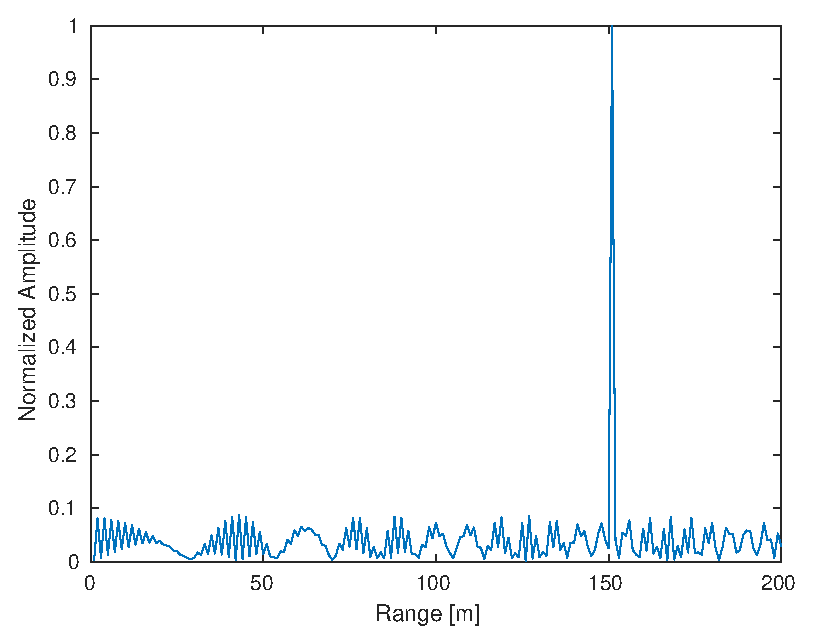
\includegraphics [width=4in]{radar_target_generation_and_detection_01.eps}


\subsection*{RANGE DOPPLER RESPONSE}

\begin{par}
The 2D FFT implementation is already provided here. This will run a 2DFFT on the mixed signal (beat signal) output and generate a range doppler map.You will implement CFAR on the generated RDM
\end{par} \vspace{1em}
\begin{verbatim}
% Range Doppler Map Generation.

% The output of the 2D FFT is an image that has reponse in the range and
% doppler FFT bins. So, it is important to convert the axis from bin sizes
% to range and doppler based on their Max values.

Mix=reshape(Mix,[Nr,Nd]);

% 2D FFT using the FFT size for both dimensions.
sig_fft2 = fft2(Mix,Nr,Nd);

% Taking just one side of signal from Range dimension.
sig_fft2 = sig_fft2(1:Nr/2,1:Nd);
sig_fft2 = fftshift (sig_fft2);
RDM = abs(sig_fft2);
RDM = 10*log10(RDM) ;

%use the surf function to plot the output of 2DFFT and to show axis in both
%dimensions
doppler_axis = linspace(-100,100,Nd);
range_axis = linspace(-200,200,Nr/2)*((Nr/2)/400);
figure('Name','2D FFT output - Range Doppler Map');
surf(doppler_axis,range_axis,RDM);
\end{verbatim}

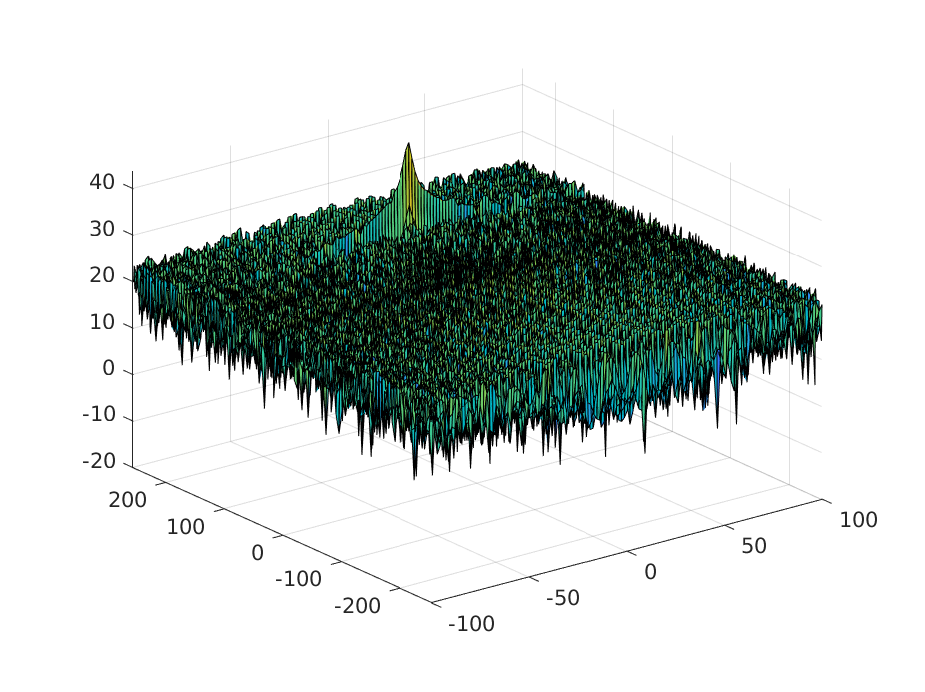
\includegraphics [width=4in]{radar_target_generation_and_detection_02.eps}


\subsection*{CFAR implementation}

\begin{verbatim}
%Slide Window through the complete Range Doppler Map

% *%TODO* :
%Select the number of Training Cells in both the dimensions.
Tr = 10;
Td = 8;

% *%TODO* :
%Select the number of Guard Cells in both dimensions around the Cell under
%test (CUT) for accurate estimation
Gr = 4;
Gd = 4;

% *%TODO* :
% offset the threshold by SNR value in dB
offset = 1.4;

% *%TODO* :
%Create a vector to store noise_level for each iteration on training cells
noise_level = zeros(1,1);


% *%TODO* :
%design a loop such that it slides the CUT across range doppler map by
%giving margins at the edges for Training and Guard Cells.
%For every iteration sum the signal level within all the training
%cells. To sum convert the value from logarithmic to linear using db2pow
%function. Average the summed values for all of the training
%cells used. After averaging convert it back to logarithimic using pow2db.
%Further add the offset to it to determine the threshold. Next, compare the
%signal under CUT with this threshold. If the CUT level > threshold assign
%it a value of 1, else equate it to 0.


% Use RDM[x,y] as the matrix from the output of 2D FFT for implementing
% CFAR
RDM = RDM/max(max(RDM));

for i = Tr+Gr+1:Nr/2-(Gr+Tr)
    for j = Td+Gd+1:Nd-(Gd+Td)
        % reset noise level for the next slide
        noise_level = zeros(1,1);
        for p = i-(Tr+Gr):i+Tr+Gr
            for q = j-(Td+Gd):j+Td+Gd
                if (abs(i-p)>Gr || abs(j-q)>Gd)
                    noise_level = noise_level + db2pow(RDM(p,q));
                end
            end
        end
        threshold = pow2db(noise_level/(2*(Td+Gd+1)*2*(Tr+Gr+1)-(Gr*Gd)-1));
        threshold = threshold + offset;
        CUT = RDM(i,j);
        if (CUT < threshold)
            RDM(i,j) = 0;
        else
            RDM(i,j) = 1;
        end
    end
end


% *%TODO* :
% The process above will generate a thresholded block, which is smaller
%than the Range Doppler Map as the CUT cannot be located at the edges of
%matrix. Hence,few cells will not be thresholded. To keep the map size same
% set those values to 0.
[rows, cols] = size(RDM);
RDM(union(1:(Tr+Gr),rows-(Tr+Gr-1):rows),:) = 0;
RDM(:,union(1:(Td+Gd),cols-(Td+Gd-1):cols)) = 0;


% *%TODO* :
%display the CFAR output using the Surf function like we did for Range
%Doppler Response output.
figure('Name','The output of the 2D CFAR process')
surf(doppler_axis,range_axis,RDM);
colorbar;
\end{verbatim}

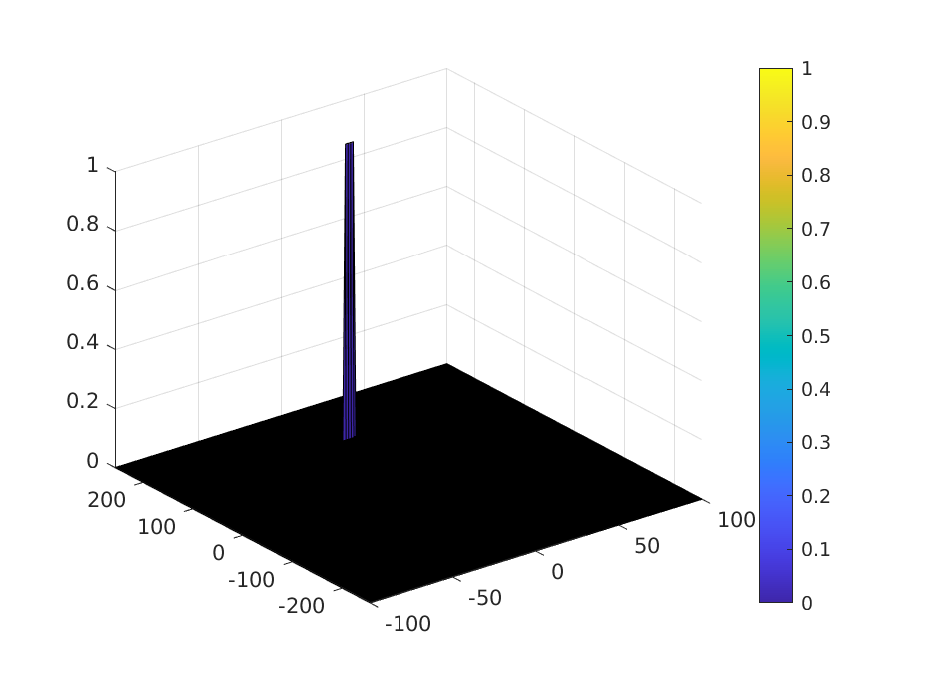
\includegraphics [width=4in]{radar_target_generation_and_detection_03.eps}



\end{document}

